% ======================================================
\documentclass[12pt,a4paper,twoside]{article}

\usepackage{geometry}
\geometry{left=1.9cm,right=1.9cm,top=1.9cm,bottom=1.9cm}

\usepackage{graphicx}
\usepackage{float}
\usepackage{xeCJK}
\usepackage{amsmath}
\usepackage{amssymb}
\usepackage{tabularx}
\usepackage{array}
\usepackage{booktabs}
\usepackage{longtable}
\usepackage{seqsplit}
\usepackage{algorithm}
\usepackage{listings}
\usepackage{tikz}
\usepackage{adjustbox}
\usepackage{pdflscape}
\usetikzlibrary{positioning,arrows.meta,fit,backgrounds}
\usepackage{xcolor}
\usepackage{xurl}
\usepackage[hidelinks]{hyperref}
\usepackage{cleveref}

\newcolumntype{L}{>{\raggedright\arraybackslash}X}
\setlength{\tabcolsep}{3pt}
\setlength{\extrarowheight}{0pt}
\setlength{\LTpre}{2pt}
\setlength{\LTpost}{5pt}

\lstset{
    language=Python,
    basicstyle=\ttfamily\footnotesize,
    columns=fullflexible,
    keepspaces=true,
    showstringspaces=false,
    breaklines=true,
    breakatwhitespace=false,
    postbreak=\mbox{\scriptsize$\hookrightarrow$\space},
}

\newcommand{\py}[1]{\lstinline{#1}}
\newcommand{\pyI}[1]{\hspace*{1.4em}\lstinline{#1}}
\newcommand{\pyII}[1]{\hspace*{2.8em}\lstinline{#1}}
\newcommand{\src}[1]{\begingroup\color{gray}\scriptsize\ttfamily\raggedright\nolinkurl{#1}\endgroup}

\title{TraceClaw: Source-Anchored Auditing of the\\
LLM Agent Control Plane}
\author{Anonymous Author(s)}
\date{October 2026}

\begin{document}
\maketitle

\begin{abstract}
Most agent evaluations focus on the final answer. TraceClaw studies a
different object: the control plane that authenticates a connection,
authorizes a method, resolves Session and Agent state, admits work, and
hands the request to the deeper runtime. We present a source-anchored
ledger for auditing this path in OpenClaw v2026.7.1-2
(\seqsplit{0790d9f593ad30c940ed93b5872a8cf6d6f3cf8c}) with a TraceClaw
instrumentation patch applied. Each Gateway stage is written as a
falsifiable claim with source anchors, case values, observation status,
and a branch outcome. In a seven-run controlled cohort, all runs cover
the same G0--G18 Gateway path (\(\mathrm{cov}=19/19\)) and directly emit
the stage outcomes (\(\mathrm{obs}=19/19\)). The result is not a broad
generalization claim. It is a controlled audit showing that source
anchoring turns successful agent executions into checkable evidence:
R1/R7 and R5/R6 repeat the same prompts with identical Gateway branches,
R2 exercises read-only retrieval, R4 exercises a local workspace
mutation, and R3 exposes an external side-effect path whose command
completed but whose downstream delivery is not verified. The paper also
separates stage-outcome observation from rationale visibility: even when
a stage outcome is observed, internal predicates and returned fields may
remain only partially visible.
\end{abstract}

\section{Introduction}
\label{sec:introduction}

An LLM agent request includes more than a model call. Before a model
answer exists, the system has already made a sequence of control-plane
decisions: whether the connection is authenticated, whether the method is
authorized, which Session and Agent own the request, whether the run is
new, whether work is admitted, and which reply resolver receives control.
These decisions are security- and reliability-relevant, yet they are easy
to hide behind a final natural-language answer.

We start from a simple concern: a final answer can be acceptable while
the path that produced it remains hard to justify. An auditor may need to
know whether an accepted request used a shared token or a device-token
fallback, whether an administrator shortcut was taken, whether
duplicate-run protection admitted or suppressed the work, or whether a
tool-side effect was approved by an explicit event or executed inside a
shell command. These questions concern the agent control plane rather
than answer quality. A screenshot of the answer or a high-level
architecture diagram usually misses them.

TraceClaw treats this control plane as the audit object. We write each
stage of a concrete request as a small checkable claim. A claim says
which source range defines the decision, which run value selected the
branch, which runtime event supports the outcome, and which nearby
branches were not taken. Ordinary tracing records what executed.
Provenance records where data or artifacts came from. TraceClaw records
why a branch was selected for one agent request, and whether that reason
is directly observed or source-derived.

TraceClaw connects tracing, provenance, and code review at the decision
boundary. A trace event without source context may show that a stage
returned \texttt{allow}, but not which predicate made the allow branch
valid. Source code without a saved run may show possible paths, but not
the one selected by the request. TraceClaw asks for the join: a source
decision site, a concrete run value, a branch outcome, and a statement
about whether the rationale is directly visible.

The study uses OpenClaw v2026.7.1-2 with a TraceClaw instrumentation
patch. The primary controlled case is R1, the prompt \texttt{How to make
a cake?}. R7 repeats that prompt under the same frozen environment. R5
and R6 repeat a tracing vs. provenance explanation prompt. R2, R3, and R4
exercise retrieval, external side effect, and local mutation paths. The
exact provenance strengths and metadata gaps are discussed in
Section~\ref{sec:experiments}.

\section{Research Questions and Contributions}
\label{sec:questions-contributions}

The paper asks three questions.

\begin{enumerate}
    \item \textbf{RQ1: Gateway path.} Can a concrete request be followed
    through all G0--G18 Gateway stages without relying on architecture
    diagrams alone?

    \item \textbf{RQ2: Evidence quality.} For each stage, what is
    directly observed, what is source-derived, and what internal rationale
    remains only partially visible?

    \item \textbf{RQ3: Runtime return.} After G18 selects the reply
    resolver, can the Agent Runtime lifecycle and the resolver return edge
    be linked back to Gateway post-processing?
\end{enumerate}

The contributions are phrased as claims plus evidence.

\begin{enumerate}
    \item \textbf{Control-plane audit framing.} We make authentication,
    authorization, Session/Agent routing, duplicate-run checks, admission,
    resolver selection, and resolver return first-class audit targets.

    \item \textbf{Source-anchored ledger.} We define a stage ledger
    \(E_i=(C_i,V_i,O_i,B_i)\), covering source anchors, concrete values,
    observation status, and branch outcome. In R1--R7, all 19 Gateway
    stages are covered and directly observed at the stage-outcome level.

    \item \textbf{Rationale-gap accounting.} We separate outcome
    observation from rationale visibility. The controlled traces expose
    all stage outcomes, but rationale visibility remains partial because
    internal predicates, stdout for short probe commands, and some return
    fields are not fully emitted.

    \item \textbf{Runtime-return analysis.} We apply the ledger idea to a
    separate AR0--AR6 runtime layer and show how no-tool, tool-using,
    local-mutation, and external side-effect executions differ without
    mixing them with historical Weather or old Cake2 traces.
\end{enumerate}

\section{Related Work}
\label{sec:related-work}

\textbf{OpenClaw architecture.}
OpenClaw architecture notes describe the broad control plane, Sessions,
Gateway, event loop, and observability goals
\cite{openclawPart1,openclawPart6,openclawExplained}. They are useful
orientation, but they are not the evidence used for stage claims. The
stage labels and branch claims in this paper are re-derived from the
pinned source and saved traces.

\textbf{Tracing and provenance.}
Dapper and OpenTelemetry make distributed execution visible through
spans and trace context \cite{dapper2010,opentelemetryTrace}. W3C PROV
offers a vocabulary for data and activity provenance \cite{provDM}. These
systems answer related but different questions. TraceClaw asks which
concrete value selected a control-plane branch and which unselected
branch is therefore excluded for this run.

This distinction matters for agent systems because many important
decisions are not naturally span-shaped. A span can record that
\texttt{chat.send} authorization completed, but the audit question is
which scope made the call legal and whether a more privileged shortcut was
skipped. A provenance relation can record that a reply depends on a tool
result, but the audit question may be whether the tool was reached after
a policy gate, a duplicate-run check, and a resolver decision. TraceClaw
therefore treats traces and provenance records as evidence sources rather
than as the complete explanation.

\textbf{Dynamic program analysis.}
Program slicing and dynamic slicing connect execution behavior to source
statements \cite{weiser1984,agrawalHorgan1990}. Dynamic invariant
detection infers likely properties from executions \cite{daikon2007}.
TraceClaw borrows the execution-specific mindset, but its output is an
audit ledger rather than a slice or an inferred invariant set.

The ledger is deliberately less automatic than slicing. It does not try
to compute all statements that influenced a value. Instead, it records the
decision sites that an auditor would cite in a paper: the source range,
the run value, the observed outcome, and the nearby branch that did not
fire. This makes the result easier to inspect, but it also means the
method depends on careful source-anchor checking and conservative
``not recorded'' labels when the trace lacks a field.

\textbf{Agent debugging and runtime observability.}
Agent debugging and visualization systems such as XAgen, FlowForge, and
visual analytics for coding agents show that process structure matters
\cite{xagen2026,wang2025illuminating,hao2025flowforge}. Runtime
observability systems such as Fangcun Observer focus on commands, file
activity, and behavior chains \cite{fangcunObserver}. TraceClaw works at
the Gateway boundary: it connects control-plane decisions to later
runtime evidence.

The closest connection to these systems is the post-G18 runtime layer.
TraceClaw does not stop when the Gateway chooses a resolver. It records
whether the deeper run is no-tool, retrieval-only, local-mutation, or an
external side-effect execution, then links the resolver-return event back
to the Gateway source path. The result is a repeatable structure for
separating control-plane evidence, runtime evidence, and source-derived
return-path claims.

\section{Method: Source-Anchored Runtime Trace}
\label{sec:method}

TraceClaw is a source-anchored auditing method for agent control planes.
It is meant for systems that are too large to print line by line, but
where a claim about execution still needs concrete evidence. The method
has four steps.

\begin{enumerate}
    \item \textbf{Choose an audited request family.} Keep one primary
    request for the full source audit, then add repeated comparison runs
    when saved traces are available. Preserve the request values that
    determine control flow, such as Session key, run ID, message, Agent
    ID, and authorization scope.

    \item \textbf{Trace the source path in execution order.} Follow the
    path from connection authentication to reply-resolver selection and
    record the handoff to the Agent Runtime.

    \item \textbf{Attach runtime evidence.} Add observed events, values,
    and timing information where the trace exposes them. When a branch is
    source-derived rather than directly logged, mark it as such.

    \item \textbf{Separate explanation from evidence.} Keep the main text
    readable, and move exact source locations, branch checks, and
    not-recorded fields to the appendix.
\end{enumerate}

The main design choice is claim-level tracing. The trace is not a prose
story written after the run; it is a set of small claims. Each stage
answers four questions: which code can execute this step, which concrete
value selects the branch, which runtime evidence supports the outcome,
and what nearby branch is ruled out for this run. Negative evidence,
such as the absence of a duplicate run or the absence of an Agent
override, is part of the audit because it often explains why the accepted
path was taken.

For one request \(r\), the Gateway path is represented as
\[
    \tau_G(r)=\langle s_0,\ldots,s_{18}\rangle .
\]
Each stage \(s_i\) has an evidence item
\[
    E_i=(C_i,V_i,O_i,B_i),
\]
where \(C_i\) is a set of source anchors, \(V_i\) contains concrete case
values, \(O_i\) is the observation status, and \(B_i\) is the branch or
outcome. A stage is covered when it has at least one verified upstream
source anchor and at least one concrete run value. It is not required
that every internal predicate, object field, or return payload field be
recorded. We report:
\[
    \mathrm{cov}(\tau_G)=
    \frac{1}{19}\sum_{i=0}^{18}
    \mathbb{1}[C_i\neq\varnothing \wedge V_i\neq\varnothing],
\]
\[
    \mathrm{obs}(\tau_G)=
    \frac{1}{19}\sum_{i=0}^{18}
    \mathbb{1}[O_i=\mathrm{Observed}].
\]
Here \(\mathrm{obs}\) measures direct stage-outcome observation. It does
not mean that every predicate, intermediate value, stdout string, token,
or returned field explaining that outcome is emitted. We therefore also
record a rationale-visibility label: \textsc{full},
\textsc{partial}, or \textsc{source-derived}. In the controlled cohort,
the Gateway outcome visibility is 19/19 for every run, while rationale
visibility is partial across stages because internal predicates and some
return fields are not fully exposed. For R1, the generated stage matrix
marks 19 of 19 Gateway stages as \textsc{partial}: every stage outcome is
observed, but none exposes all predicate-level rationale and returned
state needed for a complete semantic explanation.

The post-G18 Agent Runtime is modeled separately as AR0--AR6. AR scores
are not divided by 19. In this paper AR2 is counted as one logical stage
with an observed outcome: either observed tool start/result pairs, or
observed \texttt{no\_tool} coverage when the Agent lifecycle completes
without tool events. Tool-call-level completeness is reported separately
as \(\#\texttt{tool\_result}/\#\texttt{tool\_started}\). AR6 is marked
\textsc{source-derived}: the resolver-return event proves return to the
dispatch source point, while later Gateway post-processing is not a
separate runtime event unless instrumented.

This three-way distinction keeps the reported numbers honest. A run can
have \(\mathrm{cov}=19/19\) and \(\mathrm{obs}=19/19\) while still
containing many field-level gaps. The appendix therefore lists
\texttt{NOT RECORDED} values without lowering coverage when the stage has
enough source/value evidence to audit its outcome.

\begin{figure}[H]
\centering
\begin{adjustbox}{max width=0.94\linewidth}
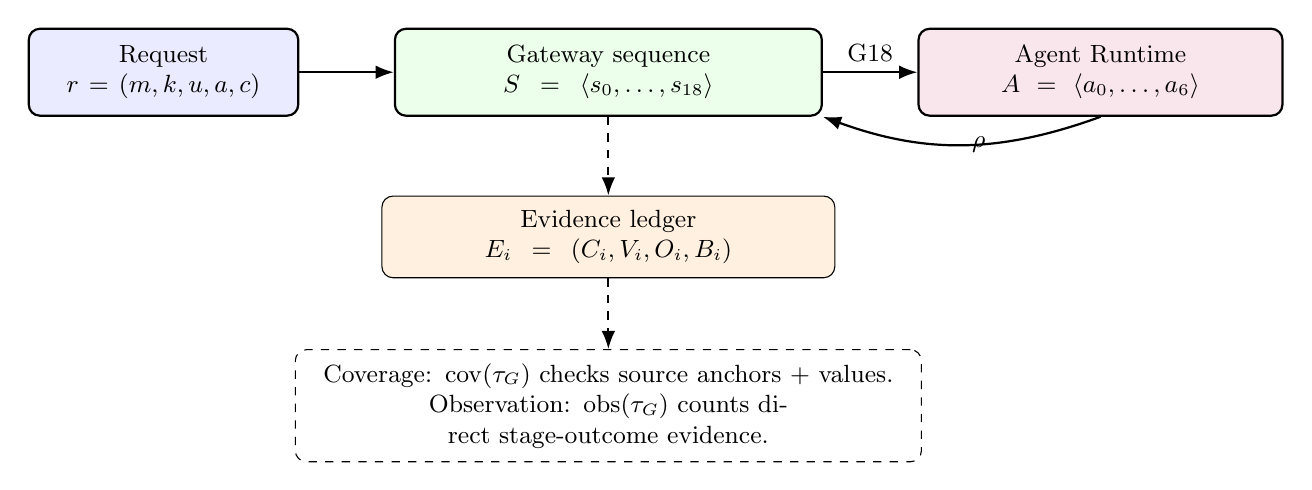
\begin{tikzpicture}[
    >=Latex,
    node distance=8mm,
    every node/.style={font=\small, align=center},
    box/.style={draw, thick, rounded corners, inner sep=6pt, minimum height=11mm},
    smallbox/.style={draw, rounded corners, inner sep=5pt, minimum height=9mm},
    note/.style={draw, dashed, rounded corners, inner sep=5pt}
]

\node[box, fill=blue!8, text width=3.0cm] (r) {Request\\\(r=(m,k,u,a,c)\)};
\node[box, fill=green!8, right=12mm of r, text width=5.0cm] (s) {Gateway sequence\\\(S=\langle s_0,\ldots,s_{18}\rangle\)};
\node[box, fill=purple!10, right=12mm of s, text width=4.2cm] (a) {Agent Runtime\\\(A=\langle a_0,\ldots,a_6\rangle\)};

\node[smallbox, fill=orange!12, below=10mm of s, text width=5.4cm] (e) {Evidence ledger\\\(E_i=(C_i,V_i,O_i,B_i)\)};
\node[note, below=9mm of e, text width=7.6cm] (scores) {Coverage: \(\mathrm{cov}(\tau_G)\) checks source anchors + values.\\
Observation: \(\mathrm{obs}(\tau_G)\) counts direct stage-outcome evidence.};

\draw[->, thick] (r) -- (s);
\draw[->, thick] (s) -- node[above]{G18} (a);
\draw[->, thick, bend left=20] (a.south) to node[right]{\(\rho\)} (s.south east);
\draw[->, thick, dashed] (s) -- (e);
\draw[->, thick, dashed] (e) -- (scores);

\end{tikzpicture}
\end{adjustbox}
\caption{Mathematical trace model. A concrete request is mapped to an
ordered Gateway stage sequence, a separate post-G18 Agent Runtime event
sequence, and an evidence ledger. The return edge \(\rho\) prevents the
analysis from stopping at resolver selection.}
\label{fig:trace-model}
\end{figure}

\subsection*{Positioning Against Common Approaches}

\small
\begin{adjustbox}{max width=\linewidth}
\begin{tabularx}{\linewidth}{
    @{}
    >{\raggedright\arraybackslash}p{0.20\linewidth}
    >{\raggedright\arraybackslash}X
    >{\raggedright\arraybackslash}X
    >{\raggedright\arraybackslash}X
    @{}
}
\toprule
\textbf{Approach} &
\textbf{What it usually shows} &
\textbf{What it misses} &
\textbf{TraceClaw difference} \\
\midrule
Architecture overview &
Main components and high-level data flow. &
Concrete branch choices, request values, and code-level evidence. &
Architecture is orientation only; every stage must map back to source and
case evidence. \\
\addlinespace
Log-only analysis &
Events emitted during one run. &
Silent branches and the source reason for each decision. &
Runtime events are aligned with source branches and negative evidence. \\
\addlinespace
Static code reading &
Possible paths in the implementation. &
Which path a real request actually took. &
The code path is bound to R1 values and runtime observations. \\
\addlinespace
Model-output evaluation &
Quality or safety of the final model response. &
Gateway admission, routing, duplicate-run handling, and resolver boundary. &
The audited object is the control path that must be trusted before the
answer is generated. \\
\bottomrule
\end{tabularx}
\end{adjustbox}
\normalsize

\section{Framework}
\label{sec:framework}

Figure~\ref{fig:framework} is the central framework of the paper. A
concrete request enters the Gateway, the Gateway is reconstructed as
ordered stage groups, and each stage is checked against a source/value
ledger. The trace then supports auditable claims about authentication,
routing, work admission, resolver selection, and runtime return.

The framework is intentionally modest. It does not summarize all
OpenClaw behavior, and it does not claim that one trace explains every
request. Its unit of analysis is narrower: one pinned source snapshot,
one ordered trace per run, and one explicit evidence ledger. The same
unit can be repeated for other prompts, compared across versions, or used
to decide where additional instrumentation is needed.

\begin{figure}[H]
\centering
\begin{adjustbox}{max width=0.96\linewidth}
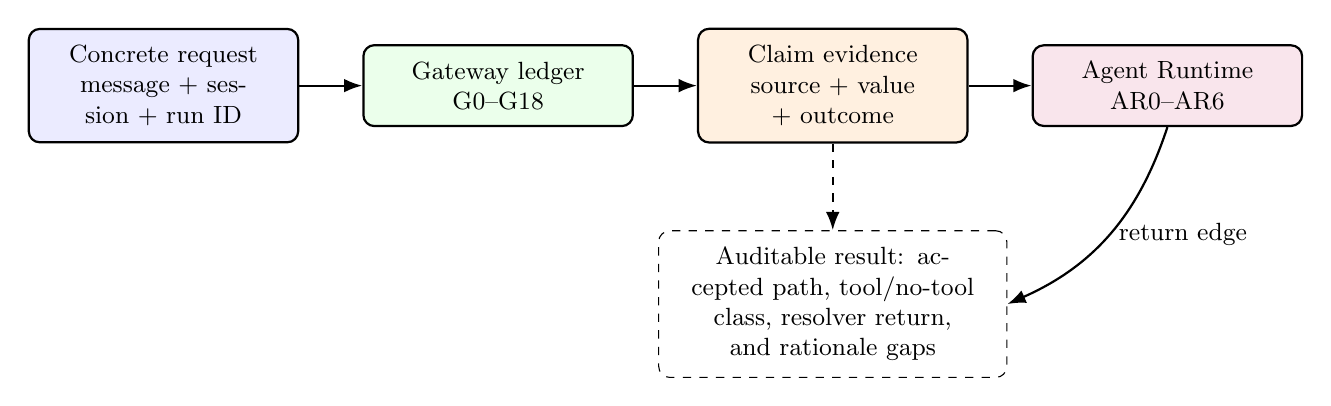
\begin{tikzpicture}[
    >=Latex,
    node distance=8mm,
    every node/.style={font=\small, align=center},
    box/.style={draw, thick, rounded corners, inner sep=6pt, text width=3.0cm},
    note/.style={draw, dashed, rounded corners, inner sep=6pt, text width=4.0cm}
]
\node[box, fill=blue!8] (req) {Concrete request\\message + session + run ID};
\node[box, fill=green!8, right=of req] (gate) {Gateway ledger\\G0--G18};
\node[box, fill=orange!12, right=of gate] (ev) {Claim evidence\\source + value + outcome};
\node[box, fill=purple!10, right=of ev] (ar) {Agent Runtime\\AR0--AR6};
\node[note, below=11mm of ev] (claim) {Auditable result: accepted path,
tool/no-tool class, resolver return, and rationale gaps};
\draw[->, thick] (req) -- (gate);
\draw[->, thick] (gate) -- (ev);
\draw[->, thick] (ev) -- (ar);
\draw[->, thick, bend left=24] (ar.south) to node[right]{return edge} (claim.east);
\draw[->, thick, dashed] (ev) -- (claim);
\end{tikzpicture}
\end{adjustbox}
\caption{TraceClaw framework. The paper separates Gateway-stage evidence
from the deeper Agent Runtime layer, then connects them with the resolver
return edge.}
\label{fig:framework}
\end{figure}

\section{Primary Controlled Case (R1)}
\label{sec:primary-case}

R1 is the controlled replacement for the old Cake2 case. Its prompt is
\texttt{How to make a cake?}. The old Cake2 artifact is kept only as
historical context because it was collected under earlier instrumentation
and used a different authentication path.

R1 is a baseline, not the main novelty by itself. The prompt is ordinary
on purpose: the value of the case is that an apparently simple accepted
request still crosses authentication, method authorization, Session
resolution, Agent selection, send policy, duplicate-run checking,
admission, context construction, resolver selection, and resolver return.
If this baseline path cannot be audited carefully, then stronger claims
about tool use or side effects would rest on a weak foundation.

R1 takes the shared-token path. G0 records token authentication material,
G1 allows the shared credential, G2 finishes with role \texttt{operator}
and scope \texttt{operator.write}, and G3 authorizes
\texttt{chat.send} through the write check. The administrator shortcut is
not an R1 claim. R1 records \texttt{hasDeviceIdentity=False}; the
device-identity and device-signature branches are therefore not used for
the R1 branch and are treated as source-derived not-taken paths. The
source establishes only this rule: if \texttt{operator.admin} is present,
authorization can short-circuit; otherwise \texttt{chat.send} requires
\texttt{operator.write}. The old Cake2 trace and R1 differ on scope, but
this paper does not claim that authentication method alone causes that
scope.

The source-anchored ledger prevents a common mistake here. The trace
directly shows the R1 branch outcome and the observed scopes. The source
explains which branches those scopes make possible. The small cohort does
not establish the causal path from authentication method to resulting
scope, so we do not state that path as a finding.

From G4 onward, R1 follows the same successful Gateway branch structure
as the later controlled runs: request validation passes, the message is
unchanged, no explicit Agent override is supplied, the Session resolves,
Agent \texttt{main} is selected, send policy allows the turn, the run is
new, work is admitted, the message context is built, and the default
\texttt{getReplyFromConfig} resolver is selected at G18. The supplementary
appendix gives the detailed per-stage source audit for R1, including source
anchors, concrete values, taken and not-taken branches, observation status,
rationale visibility, and not-recorded fields.

The baseline also fixes what the later controlled runs are compared
against. R2, R3, and R4 do not need a new Gateway theory; they reuse the
same G0--G18 ledger shape while exercising different AR classes. R5/R6
and R1/R7 then test whether exact-prompt repeats preserve the same
Gateway branch structure while changing run-specific identifiers.

\section{Deeper Agent Runtime and Return Path}
\label{sec:ar-path}

The AR layer records what happens after G18. In all seven controlled
runs, the runtime selects Agent \texttt{main}, runner \texttt{embedded},
provider \texttt{openai}, and model \texttt{gpt-5.5}. The Agent run
starts, finalizes a reply, ends with stop reason \texttt{stop}, and emits
\texttt{reply\_resolver\_returned} with a single reply result. AR6 is
then source-derived: the dispatch source resumes after the resolver
return, but the later G16/G14 post-processing is not emitted as its own
runtime event.

The AR layer uses the same audit discipline as the Gateway layer, but it
answers a different question. G0--G18 explains how the request reaches a
resolver. AR0--AR6 explains what kind of runtime execution the resolver
produces: no tool, read-only retrieval, local workspace mutation, or
external side effect. This separation prevents the paper from treating a
successful answer as the only result of interest.

\begin{table}[H]
\centering
\caption{AR-layer scores. AR2 is a logical outcome stage; no-tool runs
count the observed no-tool outcome, while tool result ratio is reported
separately.}
\label{tab:ar-metrics}
{\scriptsize
\begin{tabularx}{\linewidth}{@{}l c l c l@{}}
\toprule
Run & AR observed & AR2 outcome & Tool result ratio & AR6 \\
\midrule
R1 & 6/7 & Observed(no\_tool) & n/a & SourceDerived \\
R2 & 6/7 & Observed(tool\_results) & 6/6 & SourceDerived \\
R3 & 6/7 & Observed(tool\_results) & 5/5 & SourceDerived \\
R4 & 6/7 & Observed(tool\_results) & 4/4 & SourceDerived \\
R5 & 6/7 & Observed(no\_tool) & n/a & SourceDerived \\
R6 & 6/7 & Observed(no\_tool) & n/a & SourceDerived \\
R7 & 6/7 & Observed(no\_tool) & n/a & SourceDerived \\
\bottomrule
\end{tabularx}

}
\end{table}

R3 also exposes a rationale-level gap. The runtime records four short
capability probes using \texttt{command -v ... || true} for
\texttt{osascript}, \texttt{mutt}, \texttt{mail}, and \texttt{msmtp}.
Each exits 0, but stdout is not recorded, so the trace does not directly
show why \texttt{osascript} was chosen. The fifth command invokes Apple
Mail through \texttt{osascript} and exits 0. The evidence supports only
the host-side command completion; downstream email delivery is not
verified.

Two details make this runtime layer useful. First, a no-tool run is still
evidence: it shows that the Agent lifecycle completed without tool
events, so the absence of tools is recorded rather than assumed. Second,
tool runs are not collapsed into a single ``used tools'' flag. The paper
keeps command count, result count, stop reason, final reply, and resolver
return separate, because each supports a different claim.

\section{Controlled Experiments}
\label{sec:experiments}

\subsection{Cohort and Provenance}

The controlled cohort contains seven saved runs, R1--R7. R1--R5 come
from saved trace artifacts in the repository history. For these five
runs, the TraceClaw-side provenance is verified from repository history,
and the saved-run commits show no TraceClaw collection-code changes
within the controlled cohort. Their OpenClaw-side source identity is
reconstructed from the saved local instrumentation patch and audit notes,
because the trace payloads themselves do not embed an OpenClaw commit or
configuration fingerprint. R6 and R7 were collected later in a temporary
collection worktree. For R6/R7 only, the before and after fingerprints
directly verify the frozen environment: OpenClaw HEAD
\seqsplit{0790d9f593ad30c940ed93b5872a8cf6d6f3cf8c} and the same
instrumentation-patch hash recorded in the anonymous artifact. Between
the earlier saved-run artifact and the later repeat artifact, the only
committed changes are saved trace data and viewer cache-busting metadata.
The saved traces still do not embed the OpenClaw commit, TraceClaw
commit, or configuration fingerprint.

The table therefore should be read as a controlled cohort with two
provenance strengths. All seven runs are saved trace artifacts in the
TraceClaw repository. R6/R7 additionally have direct before/after
fingerprint evidence for the local OpenClaw checkout and patch hash.
R1--R5 are included because the repository audit found stable TraceClaw
collection code and saved trace artifacts for those runs; branch
consistency is reported below as a result, not used as an inclusion
criterion. Their OpenClaw environment is supported by post-hoc audit
rather than by trace-embedded metadata.

\begin{table}[H]
\centering
\caption{Controlled cohort. Gateway column reports coverage and direct
stage-outcome observation; tool summaries report counts rather than full
event sequences.}
\label{tab:controlled-cohort}
{\scriptsize
\begin{tabularx}{\linewidth}{@{}l X l X c c@{}}
\toprule
Run & Prompt class & Run ID & Tool summary & Gateway & AR \\
\midrule
R1 & no-tool & \texttt{8d07c88e} & none & 19/19, 19/19 & observed \\
R2 & read-only retrieval & \texttt{fba117de} & \texttt{web\_search} \( \times 6 \) & 19/19, 19/19 & observed \\
R3 & external side effect via host app & \texttt{5eb26fda} & \texttt{bash} \( \times 5 \) & 19/19, 19/19 & observed \\
R4 & local file write & \texttt{37bf6523} & \texttt{bash} \( \times 3 \) + \texttt{apply\_patch} & 19/19, 19/19 & observed \\
R5 & no-tool & \texttt{42b573dc} & none & 19/19, 19/19 & observed \\
R6 & no-tool & \texttt{3eb51151} & none & 19/19, 19/19 & observed \\
R7 & no-tool & \texttt{02225265} & none & 19/19, 19/19 & observed \\
\bottomrule
\end{tabularx}

}
\end{table}

\subsection{Gateway Coverage and Observation}

All seven controlled runs have \(\mathrm{cov}=19/19\) and
\(\mathrm{obs}=19/19\). This does not mean the traces are complete in a
strong semantic sense. It means every Gateway stage has source/value
coverage and a directly observed stage outcome. Rationale visibility is
still partial: exact internal allow sub-branches, stdout from short
probes, tokens, and some return payload fields are not fully emitted.
After re-auditing G0--G18, the final count is
\(\mathrm{full}=0/19\), \(\mathrm{partial}=19/19\), and
\(\mathrm{source\mbox{-}derived}=0/19\) for the
\texttt{rationale\_visibility} label.

\subsection{Execution Classes}

\begin{table}[H]
\centering
\caption{Execution classes assigned only from the observed runtime path.
The R3 prompt is redacted in submitted material.}
\label{tab:execution-classes}
{\scriptsize
\begin{tabularx}{\linewidth}{@{}l X l X@{}}
\toprule
Run & Prompt & Class & Observed tools \\
\midrule
R1 & How to make a cake? & no-tool & none \\
R2 & Search the web for the latest OpenTelemetry trac... & read-only retrieval & \texttt{web\_search} \( \times 6 \) \\
R3 & Draft an email to <redacted-email> saying that t... & external side effect via host app & \texttt{bash} \( \times 5 \) \\
R4 & Create a short Python script that prints the fir... & local file write & \texttt{bash} \( \times 3 \) + \texttt{apply\_patch} \\
R5 & Explain the difference between tracing and prove... & no-tool & none \\
R6 & Explain the difference between tracing and prove... & no-tool & none \\
R7 & How to make a cake? & no-tool & none \\
\bottomrule
\end{tabularx}

}
\end{table}

R1, R5, R6, and R7 are no-tool runs. R2 is read-only retrieval and records
six \texttt{web\_search} calls with matching results. R4 records
\texttt{bash}, \texttt{bash}, \texttt{apply\_patch}, and \texttt{bash},
creating a local workspace file. R3 records five \texttt{bash} calls and
is the only external side-effect path. No separate approval or
confirmation event is observed in the R3 trace. The initiating user
instruction is the only explicit user-intent context recorded for that
action.

\subsection{Read-Only Retrieval (R2)}

R2 searches for OpenTelemetry tracing documentation and summarizes it.
The runtime evidence extends beyond the final summary. The trace records
six serial \texttt{web\_search} tool calls and six matching results. The
first call searches OpenTelemetry tracing documentation; the
second opens the signals page; the third searches trace concepts; the
fourth opens the traces page; the fifth reopens the traces page; and the
sixth opens the trace SDK page. The calls run from 17:06:44.737Z to
17:07:21.532Z, followed by \texttt{agent\_reply\_finalized},
\texttt{agent\_run\_ended}, and \texttt{reply\_resolver\_returned}. This
shows how the AR layer can distinguish retrieval-heavy reasoning from a
no-tool answer even when the Gateway path is unchanged.

R2 keeps the control plane constant while changing the runtime class.
G0--G18 still authenticate, authorize, admit, and route the request
through the same successful structure. The difference appears after G18:
AR2 contains retrieval tool activity and matching tool results. A
Gateway-only ledger can say how the request reached the resolver. The AR
layer shows that the answer used external retrieval events rather than
model-only generation.

\subsection{Local Mutation (R4)}

R4 asks for a short Python script that prints Fibonacci numbers. The AR
ledger records a four-step local sequence: \texttt{pwd}, \texttt{rg
--files}, an \texttt{apply\_patch} add of \texttt{fibonacci.py}, and
\texttt{python3 fibonacci.py}. The observed tool window runs from
17:08:57.709Z to 17:09:07.329Z. The mutation is local to the workspace.
The claim is therefore narrower than ``the agent can edit arbitrary
files'': in this run, the saved trace shows a local workspace write and
subsequent runtime completion.

R4 separates permission from effect. The Gateway permits a normal
\texttt{chat.send} request; it does not by itself describe the later
workspace mutation. The AR ledger records the mutation as a concrete tool
sequence, including the post-mutation check. The claim stays narrow: the
evidence is local, saved, and tied to this workspace trace.

\subsection{External Side Effect (R3)}

R3 requests an email draft-and-send action. The trace records four
concurrent capability probes, then one \texttt{osascript} invocation of
Apple Mail. The host-side send command completed with exit code 0; the
trace does not verify downstream delivery. The final assistant reply says
more than the trace can prove. The trace directly observes \texttt{bash}
execution. The effective tool-policy path that allows that execution is
source-derived from the G16 dispatch path, not emitted as a separate
authorization event in the saved trace.

R3 gives the clearest rationale-visibility gap. The runtime records that
the command completed, but it does not record stdout from the short
\texttt{command -v ... || true} probes and it does not emit a separate
approval or delivery-confirmation event. A normal success log might
invite a downstream-delivery inference. The ledger supports the weaker
claim: the host-side command path completed, and the missing
approval/delivery evidence is an observability gap.

\subsection{Exact-Prompt Repeatability}

\begin{table}[H]
\centering
\caption{Exact-prompt repeatability checks.}
\label{tab:repeatability}
{\scriptsize
\begin{tabularx}{\linewidth}{@{}l l c c c c@{}}
\toprule
Pair & G0--G18 branch diff & Agent & Resolver & Tools & AR structure \\
\midrule
R1/R7 & none & yes & yes & yes & yes \\
R5/R6 & none & yes & yes & yes & yes \\
\bottomrule
\end{tabularx}

}
\end{table}

R1/R7 and R5/R6 repeat exact prompts. In both pairs, G0--G18 branches,
Agent, resolver, tool/no-tool choice, stop reason, and AR structure match.
The expected differences are run ID, Gateway Session key, AR session
identifier where emitted, timestamps, and reply wording.

The repeat pairs are not a general stability theorem. They are a sanity
check on the ledger. If the same prompt under the same controlled
environment changed Gateway branches without a recorded reason, the stage
model would be suspect. Instead, the branch structure is stable and the
run-specific identifiers change as expected. This supports using R1 as
the detailed source-audit baseline while using R7 as an exact-prompt
repeat.

\subsection{Historical Weather Supplement}
\label{sec:historical-weather}

The repository also contains historical Weather traces collected under
earlier instrumentation. We keep them outside the R1--R7 quantitative
cohort. They are useful only as qualitative replication evidence: the
successful Weather requests follow a comparable G0--G18 Gateway skeleton,
while their post-G18 tool paths vary. The New York Weather evidence
contains six saved traces with near-identical prompts rather than exact
prompt repeats. Four use only \texttt{web\_search}; two contain a
\texttt{bash} setup or skill-loading step followed by \texttt{web\_search}.
A separate Beijing Weather trace also contains \texttt{bash} followed by
\texttt{web\_search}. We do not mix the Beijing trace into the New York
count, and no Weather score is combined with R1--R7.

\begin{table}[H]
\centering
\caption{Historical Weather evidence kept as supplementary context. The
counts come from saved repository artifacts, not from new runs.}
\label{tab:historical-weather}
{\scriptsize
\begin{tabularx}{\linewidth}{@{}l c X X X@{}}
\toprule
Evidence set & Saved runs & Prompt relationship & Observed post-G18 tool pattern & Role in this paper \\
\midrule
New York Weather & 6 & near-identical Weather requests & 4 \(\times\) \texttt{web\_search}; 2 \(\times\) \texttt{bash} + \texttt{web\_search} & historical qualitative replication only \\
Beijing Weather & 1 & separate Weather request & \texttt{bash} + \texttt{web\_search} & separate historical example; excluded from New York count \\
\bottomrule
\end{tabularx}
}
\end{table}

\subsection{Repeated-Run Consistency and Rationale Gaps}

All 19 Gateway stages take the same branch across R1--R7. The values
that should differ do differ: run identifiers, Session keys, timestamps,
and the AR-layer tool path. Because every Gateway stage still has only
\textsc{partial} rationale visibility, the compact main-paper table lists
the gaps that matter instead of printing 19 rows with the same visibility
label. The full stage-by-run matrix and the R1 per-stage source audit are
kept in the supplementary appendix.

\begin{table}[H]
\centering
\caption{Representative rationale-level gaps in the controlled cohort.
Each listed Gateway stage has an observed outcome, but not every internal
predicate or returned field is emitted.}
\label{tab:rationale-gaps}
{\scriptsize
\begin{tabularx}{\linewidth}{@{}l X X@{}}
\toprule
Stage(s) & Observed outcome & Rationale field not fully emitted \\
\midrule
G0/G2 & shared-token authentication succeeds; device-token path is not used &
concrete device-token candidate source and device-signature subpath \\
G3 & \texttt{chat.send} is allowed through \texttt{operator.write} &
\texttt{auth\_reason}; administrator shortcut exclusion is source-derived from scopes \\
G7/G8/G12 & Session resolves, Agent/Session validation passes, work is admitted &
persistent store details, full Session object, and admission internals \\
G10 & send policy outcome is \texttt{allow} &
exact internal allow sub-branch and policy-rule rationale \\
G14/G16/G18 & dispatch enters auto-reply, normal path continues, resolver is selected &
full dispatch/reply payloads and post-return Gateway state \\
AR/R3 & five \texttt{bash} tools complete with exit code 0 &
probe stdout, separate approval event, and delivery confirmation \\
\bottomrule
\end{tabularx}
}
\end{table}

\subsection{Audit Findings}

The controlled cohort yields three findings that plain final-answer
evaluation would miss. First, Gateway structure is stable across seven
successful runs while runtime class varies. Second, R3 exposes an
approval and tool-policy audit boundary: the trace records \texttt{bash}
execution and command completion, while the effective policy path that
permits the tool is source-derived and no separate delivery-confirmation
event is recorded. Third, the traces demonstrate a rationale-level
observability gap even with 19/19 stage outcome observation.

These findings are modest but specific. TraceClaw does not show that
OpenClaw is safe in general, nor that a successful run proves policy
compliance in every layer. It shows that an accepted request can be
turned into a falsifiable ledger: G3 can prove that the ordinary
\texttt{operator.write} branch, not the administrator shortcut, is the R1
authorization path; G10 can show the outcome \texttt{allow} while still
leaving the exact internal allow sub-branch only partially visible; AR6
can show resolver return while marking later Gateway resume as
source-derived. Final-answer evaluation alone would not expose these
control-flow and evidence-boundary details.

\subsection{Coverage Limits}

The cohort is small, successful, same-machine, and same-configuration. It
does not cover rejected, failed, retried, cancelled, cross-version, or
multi-framework paths. Weather runs and the old Cake2 trace are historical
notes only. They are useful for artifact continuity, but they are not
mixed into the R1--R7 quantitative tables.

The controlled runs also share the same broad authorization shape:
shared-token authentication, role \texttt{operator}, and ordinary
\texttt{operator.write} authorization for \texttt{chat.send}. This is
good for controlled comparison, but it leaves other policy branches
untested. The historical Cake2 artifact remains useful because it shows a
different authentication/scope combination, yet it is not used as a
current quantitative baseline because it predates later collector
changes.

\section{Limitations}
\label{sec:limitations}

The evidence supports a controlled audit of seven successful requests,
not a broad claim about all OpenClaw behavior. The runs share one local
configuration and one instrumented OpenClaw source tree. Because the
traces do not embed commit or configuration fingerprints, provenance has
to be reconstructed from repository history and audit notes.

This provenance limit affects the strength of the claims. A stronger
artifact would store \texttt{openclawCommit}, \texttt{traceclawCommit},
trace schema version, configuration fingerprint, and instrumentation
patch hash inside every trace. Without that embedded metadata, we can
audit saved behavior, but we must describe provenance strength carefully.
R6/R7 have direct before/after fingerprint checks; R1--R5 are supported
by saved trace artifacts and repository history plus post-hoc OpenClaw
patch audit.

The method is also partly manual. Stage labels are introduced by
TraceClaw, not by OpenClaw itself, and source anchors require content
checking. The appendix therefore cites upstream 0790d9f decision sites,
not patched instrumentation line numbers. This is deliberate: runtime
events may be emitted by instrumentation, but the branch claim should
point to the upstream decision it observes.

Finally, the external side-effect case is intentionally conservative. The
trace proves that a host-side command exited successfully; it does not
prove email delivery. The paper therefore treats R3 as an audit finding
about command-level evidence and missing approval/confirmation events,
not as proof of downstream delivery.

\section{Artifact, Privacy, and Future Work}
\label{sec:artifact}

The artifact contains the viewer, saved traces, generated controlled
tables, and a sanitized instrumentation patch reference. For double-blind
submission, author-identifying URLs, personal email addresses, hostnames,
usernames, and absolute local paths should be removed or replaced by
anonymous placeholders. The working \texttt{artifacts/audit/} directory is
not a submission bundle. If any audit-derived file is copied into a
submitted artifact, it must be redacted under the same rules.

Future work should add commit/config fingerprints directly to every trace,
rerun failure and rejection paths, and build an interactive evidence graph
that links each stage to source anchors, runtime events, and case values.
The next cohort should include rejected authentication, failed
authorization, duplicate-run suppression, cancelled execution, tool
policy denial, and cross-version replay. Those cases would test whether
the ledger remains useful when the path stops early or changes shape.

\begin{thebibliography}{99}

\bibitem{dapper2010}
Benjamin H. Sigelman, Luiz Andre Barroso, Mike Burrows, Pat Stephenson,
Manoj Plakal, Donald Beaver, Saul Jaspan, and Chandan Shanbhag. Dapper,
a Large-Scale Distributed Systems Tracing Infrastructure. Google
Technical Report dapper-2010-1, 2010.

\bibitem{opentelemetryTrace}
OpenTelemetry. Trace API Specification.
\url{https://opentelemetry.io/docs/specs/otel/trace/api/}. Accessed 2026-09-30.

\bibitem{provDM}
Luc Moreau and Paolo Missier, editors. PROV-DM: The PROV Data Model. W3C
Recommendation, 30 April 2013.

\bibitem{weiser1984}
Mark Weiser. Program slicing. IEEE Transactions on Software Engineering,
SE-10(4):352--357, 1984.

\bibitem{agrawalHorgan1990}
Hiralal Agrawal and Joseph R. Horgan. Dynamic program slicing. In
Proceedings of the ACM SIGPLAN Conference on Programming Language Design
and Implementation, 1990.

\bibitem{daikon2007}
Michael D. Ernst, Jeff H. Perkins, Philip J. Guo, Stephen McCamant,
Carlos Pacheco, Matthew S. Tschantz, and Chen Xiao. The Daikon system for
dynamic detection of likely invariants. Science of Computer Programming,
69(1--3):35--45, 2007.

\bibitem{xagen2026}
XAgen: An Explainability Tool for Identifying and Correcting Failures in
Multi-Agent Workflows. \url{https://arxiv.org/abs/2512.17896}. Accessed 2026-09-24.

\bibitem{wang2025illuminating}
Illuminating LLM Coding Agents: Visual Analytics for Deeper Understanding
and Enhancement. \url{https://arxiv.org/abs/2508.12555}. Accessed 2026-09-24.

\bibitem{hao2025flowforge}
FlowForge: Guiding the Creation of Multi-agent Workflows with Interactive
Visualizations as a Thinking Scaffold. IEEE VIS 2025 program page.

\bibitem{fangcunObserver}
Fangcun Observer: Runtime Security for AI Agents.
\url{https://fangcunleap.com/blog/observer}. Accessed 2026-09-24.

\bibitem{openclawPart1}
OpenClaw Architecture - Part 1: Control Plane, Sessions, and the Event Loop.
\url{https://theagentstack.substack.com/p/openclaw-architecture-part-1-control}.
Accessed 2026-09-24.

\bibitem{openclawPart6}
OpenClaw Architecture - Part 6: Reliability, Observability, and Evaluation.
\url{https://theagentstack.substack.com/p/openclaw-architecture-part-6-reliability}.
Accessed 2026-09-24.

\bibitem{openclawExplained}
OpenClaw Architecture, Explained: How It Works as an OS for AI Agents.
\url{https://ppaolo.substack.com/p/openclaw-system-architecture-overview}.
Accessed 2026-09-24.

\bibitem{traceclawArtifact}
Anonymous. TraceClaw Anonymous Artifact. Anonymized artifact submitted as
supplementary material.

\end{thebibliography}

\end{document}
